\documentclass[11pt]{article}
% ===========================================================================
%  Shared preamble for all MPM2D worksheets — input right after \documentclass.
%  (Files beginning with "_" are skipped by mpm2d-worksheet-publish.mjs.)
% ===========================================================================
\usepackage[letterpaper,top=2.2cm,bottom=1.9cm,left=1.6cm,right=1.6cm,headheight=28pt,footskip=24pt]{geometry}
\usepackage{amsmath,amssymb}
\usepackage[T1]{fontenc}
\usepackage[utf8]{inputenc}
\usepackage{lmodern}
\usepackage{xcolor}
\usepackage[most]{tcolorbox}
\usepackage{enumitem}
\usepackage{multicol}
\usepackage{fancyhdr}
\usepackage{tikz}
\usetikzlibrary{calc}
\usepackage{pgfplots}
\pgfplotsset{compat=1.18}

\definecolor{exblue}{HTML}{4A90E2}
\definecolor{exbg}{HTML}{E6F3FF}
\definecolor{qorange}{HTML}{E69138}
\definecolor{qbg}{HTML}{FFF7CC}
\definecolor{keygray}{HTML}{475569}
\definecolor{keybg}{HTML}{F1F5F9}
\definecolor{iagreen}{HTML}{14653B}
\definecolor{titleblue}{HTML}{1D4ED8}
% Rotating palette so each worked example gets its own colour.
\definecolor{ex0}{HTML}{2563A0}\definecolor{ex1}{HTML}{3B7D3B}\definecolor{ex2}{HTML}{8A5A00}
\definecolor{ex3}{HTML}{A3327A}\definecolor{ex4}{HTML}{6D28A3}\definecolor{ex5}{HTML}{B08900}
\definecolor{ex6}{HTML}{0E7490}\definecolor{ex7}{HTML}{9A3412}\definecolor{ex8}{HTML}{15803D}

\pagestyle{fancy}
\fancyhf{}
\fancyhead[L]{\footnotesize NAME: \underline{\hspace{3.4cm}}}
\fancyhead[C]{\textbf{Integration Academy}\\[-2pt]{\scriptsize Math Simplified \textperiodcentered{} Success Amplified}}
\fancyhead[R]{\footnotesize MPM2D}
\fancyfoot[L]{\scriptsize dr.merie@IntegrationAcademy.ca}
\fancyfoot[C]{\scriptsize\thepage}
\fancyfoot[R]{\scriptsize IntegrationAcademy.ca}
\renewcommand{\headrulewidth}{1.2pt}
\renewcommand{\footrulewidth}{0.4pt}
\setlength{\parindent}{0pt}
\setlength{\parskip}{4pt}

% Examples are NOT breakable, so each example + its solution stays on one page.
\newtcolorbox{example}[2]{colframe=#1,colback=#1!7,coltitle=white,colbacktitle=#1,fonttitle=\bfseries,title={#2},arc=3pt,boxrule=1pt}
\newtcolorbox{qbox}[1]{colframe=qorange,colback=qbg,coltitle=white,colbacktitle=qorange,fonttitle=\bfseries,title={#1},arc=3pt,breakable,boxrule=1pt}
\newtcolorbox{keybox}{colframe=keygray,colback=keybg,coltitle=white,colbacktitle=keygray,fonttitle=\bfseries,title={$\checkmark$\ Answer Key},arc=3pt,breakable,boxrule=1pt}
\newtcolorbox{recapbox}{colframe=keygray,colback=keybg,coltitle=white,colbacktitle=keygray,fonttitle=\bfseries,title={Question Recap},arc=3pt,breakable,boxrule=1pt}
\newtcolorbox{ideabox}{colframe=titleblue,colback=titleblue!6,coltitle=white,colbacktitle=titleblue,fonttitle=\bfseries,title={The Big Ideas},arc=3pt,breakable,boxrule=1.2pt}
\newtcolorbox{learnbox}{colframe=iagreen,colback=iagreen!5,coltitle=white,colbacktitle=iagreen,fonttitle=\bfseries,title={Core Concepts},arc=3pt,breakable,boxrule=1.2pt}
\newcommand{\lh}[1]{\par\smallskip{\bfseries\color{iagreen}#1}\par\nobreak\smallskip}

\newcommand{\soln}{\par\smallskip\textit{\textbf{Solution.}}\ }
\newcommand{\workspace}[1]{\par\vspace{3pt}\fcolorbox{black!30}{white}{\begin{minipage}[t][#1][t]{\dimexpr\linewidth-2\fboxsep\relax}\ \end{minipage}}\par}
\newcommand{\sech}[1]{\par\vspace{8pt}{\Large\bfseries\color{iagreen}#1}\par\nobreak\vspace{2pt}{\color{black!20}\hrule height1pt}\vspace{6pt}}

% A compact coordinate plot sized for an example box: \eplot{xmin}{xmax}{ymin}{ymax}{body}
\newcommand{\eplot}[5]{\begin{center}\begin{tikzpicture}
\begin{axis}[width=6.8cm,height=4.4cm,axis lines=middle,xlabel={\tiny$x$},ylabel={\tiny$y$},
grid=both,grid style={gray!16},xmin=#1,xmax=#2,ymin=#3,ymax=#4,
xtick distance=2,ytick distance=2,tick label style={font=\tiny},axis line style={-},samples=120]
#5
\end{axis}\end{tikzpicture}\end{center}}

% Same as \eplot but with its own tick spacing: \eplotx{xmin}{xmax}{ymin}{ymax}{xtick}{ytick}{body}
\newcommand{\eplotx}[7]{\begin{center}\begin{tikzpicture}
\begin{axis}[width=8.4cm,height=5.4cm,axis lines=middle,xlabel={\tiny$x$},ylabel={\tiny$y$},
grid=both,grid style={gray!16},xmin=#1,xmax=#2,ymin=#3,ymax=#4,
xtick distance=#5,ytick distance=#6,tick label style={font=\tiny},axis line style={-},samples=120]
#7
\end{axis}\end{tikzpicture}\end{center}}

% A sine-curve plot (degrees on x, 0..360): \splot{ymin}{ymax}{body}
\newcommand{\splot}[3]{\begin{center}\begin{tikzpicture}
\begin{axis}[width=8.6cm,height=4.6cm,axis lines=middle,xlabel={\tiny$x\,(^\circ)$},ylabel={\tiny$y$},
grid=both,grid style={gray!16},xmin=0,xmax=360,ymin=#1,ymax=#2,
xtick distance=90,ytick distance=1,tick label style={font=\tiny},axis line style={-},samples=180]
#3
\end{axis}\end{tikzpicture}\end{center}}

% A small coordinate plot: \plot{xmin}{xmax}{ymin}{ymax}{body}
\newcommand{\plot}[5]{\begin{center}\begin{tikzpicture}
\begin{axis}[width=8.4cm,height=6cm,axis lines=middle,xlabel={\scriptsize$x$},ylabel={\scriptsize$y$},
grid=both,grid style={gray!16},xmin=#1,xmax=#2,ymin=#3,ymax=#4,
xtick distance=2,ytick distance=2,tick label style={font=\tiny},axis line style={-}]
#5
\end{axis}\end{tikzpicture}\end{center}}

% Right triangle (angle theta at bottom-left, right angle at bottom-right):
%   \rtri{drawBase}{drawHeight}{oppLabel}{adjLabel}{hypLabel}
\newcommand{\rtri}[5]{\begin{center}\begin{tikzpicture}[scale=0.85]
\coordinate (A) at (0,0);\coordinate (B) at (#1,0);\coordinate (C) at (#1,#2);
\draw[thick,exblue] (A)--(B)--(C)--cycle;
\draw[black] ($(B)+(-0.32,0)$)--($(B)+(-0.32,0.32)$)--($(B)+(0,0.32)$);
\node[below] at ($(A)!0.5!(B)$){#4};
\node[right] at ($(B)!0.5!(C)$){#3};
\node[above left] at ($(A)!0.5!(C)$){#5};
\node at (0.7,0.22){$\theta$};
\end{tikzpicture}\end{center}}

% General (oblique) triangle with vertex labels and opposite-side labels:
%   \gtri{Alabel}{Blabel}{Clabel}{aSide}{bSide}{cSide}
\newcommand{\gtri}[6]{\begin{center}\begin{tikzpicture}[scale=0.85]
\coordinate (A) at (0,0);\coordinate (B) at (5,0);\coordinate (C) at (1.6,3);
\draw[thick,exblue] (A)--(B)--(C)--cycle;
\node[below left] at (A){#1};\node[below right] at (B){#2};\node[above] at (C){#3};
\node[below] at ($(A)!0.5!(B)$){#6};
\node[right] at ($(B)!0.5!(C)$){#4};
\node[left] at ($(A)!0.5!(C)$){#5};
\end{tikzpicture}\end{center}}

\fancyhead[R]{\footnotesize MHF4U \textperiodcentered{} 5.1}
\begin{document}

\begin{center}
{\LARGE\bfseries\color{titleblue}Worksheet 5.1 --- Radian Measure}\\[2pt]
{\small Grade 12 Advanced Functions (MHF4U) \textperiodcentered{} Unit 5: Trigonometric Functions}
\end{center}

\begin{ideabox}
A radian measures an angle by arc length; a full turn is $2\pi$ radians $=360^\circ$. Convert with $\tfrac{\pi}{180}$ or $\tfrac{180}{\pi}$, and use $s=r\theta$ for arc length.
\begin{itemize}[leftmargin=*,itemsep=2pt]
  \item Degrees$\to$radians: $\times\tfrac{\pi}{180}$. Radians$\to$degrees: $\times\tfrac{180}{\pi}$.
  \item $30^\circ=\tfrac{\pi}{6},\ 45^\circ=\tfrac{\pi}{4},\ 60^\circ=\tfrac{\pi}{3},\ 90^\circ=\tfrac{\pi}{2}$.
  \item Arc length $s=r\theta$ ($\theta$ in radians).
\end{itemize}
\end{ideabox}

\begin{learnbox}
\lh{A natural angle unit}A \textbf{radian} measures an angle by arc length: one radian subtends an arc equal to the radius, and a full circle is $2\pi$ radians.
\lh{Converting}Since $180^\circ=\pi$ radians, convert by multiplying by $\dfrac{\pi}{180^\circ}$ or $\dfrac{180^\circ}{\pi}$ as needed.
\lh{Arc and sector}In radians the formulas simplify: arc length is $r\theta$ and sector area is $\tfrac12 r^2\theta$.
\end{learnbox}

\sech{Worked Examples}

\begin{example}{ex0}{Example 1 --- Degrees to radians}
Convert $180^\circ$ to radians.\soln $180\cdot\tfrac{\pi}{180}=\pi$. Radians are the natural axis for trig graphs:\begin{center}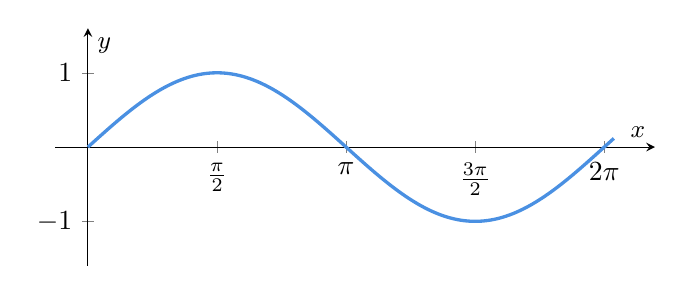
\begin{tikzpicture}\begin{axis}[width=9.2cm,height=4.6cm,axis lines=middle,xlabel={\small$x$},ylabel={\small$y$},xmin=-0.4,xmax=6.9,ymin=-1.6,ymax=1.6,samples=220,xtick={1.5708,3.1416,4.7124,6.2832},xticklabels={$\frac{\pi}{2}$,$\pi$,$\frac{3\pi}{2}$,$2\pi$}]\addplot[exblue,very thick,domain=0:6.4]{sin(deg(x))};\end{axis}\end{tikzpicture}\end{center}
\end{example}

\begin{example}{ex1}{Example 2 --- Degrees to radians}
Convert $90^\circ$ to radians.\soln $90\cdot\tfrac{\pi}{180}=\tfrac{\pi}{2}$.
\end{example}

\begin{example}{ex2}{Example 3 --- Radians to degrees}
Convert $\tfrac{5\pi}{4}$ to degrees.\soln $\tfrac{5\pi}{4}\cdot\tfrac{180}{\pi}=225^\circ$.
\end{example}

\begin{example}{ex3}{Example 4 --- Degrees to radians}
Convert $45^\circ$ to radians.\soln $45\cdot\tfrac{\pi}{180}=\tfrac{\pi}{4}$.
\end{example}

\begin{example}{ex4}{Example 5 --- Arc length}
Arc length for $r=8,\ \theta=\tfrac{\pi}{4}$.\soln $s=r\theta=8\cdot\tfrac{\pi}{4}=2\pi$.
\end{example}

\begin{example}{ex5}{Example 6 --- Degrees to radians}
Convert $15^\circ$ to radians.\soln $15\cdot\tfrac{\pi}{180}=\tfrac{\pi}{12}$.
\end{example}

\begin{example}{ex6}{Example 7 --- Radians to degrees}
Convert $\tfrac{\pi}{5}$ to degrees.\soln $\tfrac{\pi}{5}\cdot\tfrac{180}{\pi}=36^\circ$.
\end{example}

\begin{example}{ex7}{Example 8 --- Degrees to radians}
Convert $300^\circ$ to radians.\soln $300\cdot\tfrac{\pi}{180}=\tfrac{5\pi}{3}$.
\end{example}

\begin{example}{ex8}{Example 9 --- Arc length}
Arc length for $r=12,\ \theta=\tfrac{\pi}{6}$.\soln $s=12\cdot\tfrac{\pi}{6}=2\pi$.
\end{example}

\clearpage
\sech{Your Turn --- Show Your Work}
For each question, show all steps clearly in the space provided.

\begin{qbox}{Question 1}
Convert $20^\circ$ to radians.\workspace{2.4cm}
\end{qbox}

\begin{qbox}{Question 2}
Convert $\tfrac{11\pi}{12}$ to degrees.\workspace{2.4cm}
\end{qbox}

\begin{qbox}{Question 3}
Convert $80^\circ$ to radians.\workspace{2.4cm}
\end{qbox}

\begin{qbox}{Question 4}
Convert $\tfrac{7\pi}{9}$ to degrees.\workspace{2.4cm}
\end{qbox}

\begin{qbox}{Question 5}
Arc length for $r=9,\ \theta=\tfrac{2\pi}{3}$?\workspace{2.4cm}
\end{qbox}

\begin{qbox}{Question 6}
Convert $40^\circ$ to radians.\workspace{2.4cm}
\end{qbox}

\begin{qbox}{Question 7}
Convert $\tfrac{5\pi}{9}$ to degrees.\workspace{2.4cm}
\end{qbox}

\begin{qbox}{Question 8}
Convert $450^\circ$ to radians.\workspace{2.4cm}
\end{qbox}

\begin{qbox}{Question 9}
Arc length for $r=20,\ \theta=\tfrac{\pi}{4}$?\workspace{2.4cm}
\end{qbox}

\begin{qbox}{Question 10}
Convert $12^\circ$ to radians.\workspace{2.4cm}
\end{qbox}

\begin{qbox}{Question 11}
Convert $\tfrac{3\pi}{5}$ to degrees.\workspace{2.4cm}
\end{qbox}

\begin{qbox}{Question 12}
Convert $105^\circ$ to radians.\workspace{2.4cm}
\end{qbox}

\begin{qbox}{Question 13 --- Challenge}
A wheel of radius 0.5 m turns through $4\pi$ radians. How far does a point on the rim travel?\workspace{3cm}
\end{qbox}

\clearpage
\sech{Question Recap \& Answer Key}

\begin{recapbox}
\begin{multicols}{2}
\small
\begin{enumerate}[leftmargin=*,itemsep=3pt]
  \item Convert $20^\circ$ to radians.
  \item Convert $\tfrac{11\pi}{12}$ to degrees.
  \item Convert $80^\circ$ to radians.
  \item Convert $\tfrac{7\pi}{9}$ to degrees.
  \item Arc length for $r=9,\ \theta=\tfrac{2\pi}{3}$?
  \item Convert $40^\circ$ to radians.
  \item Convert $\tfrac{5\pi}{9}$ to degrees.
  \item Convert $450^\circ$ to radians.
  \item Arc length for $r=20,\ \theta=\tfrac{\pi}{4}$?
  \item Convert $12^\circ$ to radians.
  \item Convert $\tfrac{3\pi}{5}$ to degrees.
  \item Convert $105^\circ$ to radians.
  \item A wheel of radius 0.5 m turns through $4\pi$ radians. How far does a point on the rim travel?
\end{enumerate}
\end{multicols}
\end{recapbox}

\begin{keybox}
\begin{multicols}{2}
\small
\begin{enumerate}[leftmargin=*,itemsep=3pt]
  \item $\tfrac{\pi}{9}$
  \item $165^\circ$
  \item $\tfrac{4\pi}{9}$
  \item $140^\circ$
  \item $6\pi$
  \item $\tfrac{2\pi}{9}$
  \item $100^\circ$
  \item $\tfrac{5\pi}{2}$
  \item $5\pi$
  \item $\tfrac{\pi}{15}$
  \item $108^\circ$
  \item $\tfrac{7\pi}{12}$
  \item $s=0.5\cdot4\pi=2\pi\approx6.28$ m
\end{enumerate}
\end{multicols}
\end{keybox}

\end{document}
